\CedricSpeak{}
\subsection{La méthodologie}
\begin{frame}{Quelques chiffres\ldots}
	\begin{block}{Github}
		\begin{tabular}{cc}
			\hspace{-20px}
			\begin{minipage}{0.56\textwidth}
				\begin{itemize}
					\item 
\includegraphics[height=10px]{images/labels/pullRequestGreen.JPG}~Pull Requests~
\includegraphics[height=10px]{images/stats/pullrequest.png}
					\item 
\includegraphics[height=10px]{images/labels/issues.JPG}~Issues~
\includegraphics[height=10px]{images/stats/issues.png}
				\end{itemize}
			\end{minipage}
			\hspace{-15px}
			\begin{minipage}{0.5\textwidth}
				\begin{itemize}
					\item 
\includegraphics[height=10px]{images/labels/branches.JPG}~Branches~
\includegraphics[height=10px]{images/stats/branches.png}
					\item 
\includegraphics[height=10px]{images/labels/commits.JPG}~Commits~
\includegraphics[height=10px]{images/stats/commits.png}
				\end{itemize}
			\end{minipage}
		\end{tabular}
	\end{block}
	\pause
	\begin{block}{Scrum}
		\begin{itemize}
			\item 54 User stories
			\item 6 sprints
			\item 2 releases
		\end{itemize}
	\end{block}
	\pause
	\begin{block}{Code}
		\begin{itemize}
			\item Nombre de lignes 
\includegraphics[height=9px]{images/stats/nblines.jpg}
			\item 
\includegraphics[height=7px]{images/coverage.png}~~
\includegraphics[height=7px]{images/build.png}
			\item Pourcentage documentation
		\end{itemize}
	\end{block}

\end{frame}

\begin{frame}{BurnUp Chart}
	\begin{figure}[H]
		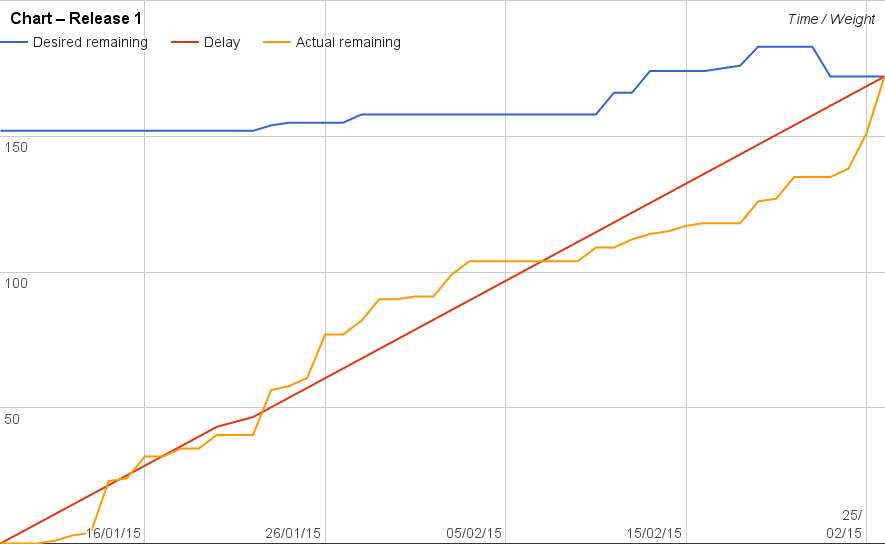
\includegraphics[width=9.5cm]{images/release1Chart.png}
		\caption{Première release}
	\end{figure}
\end{frame}

\TsooSpeak{}
\subsection{Le logiciel}
\begin{frame}{Quelques captures d'écrans\ldots}
	\begin{figure}[H]
		\centering
		\vspace{-15px}
		\only<1>{
		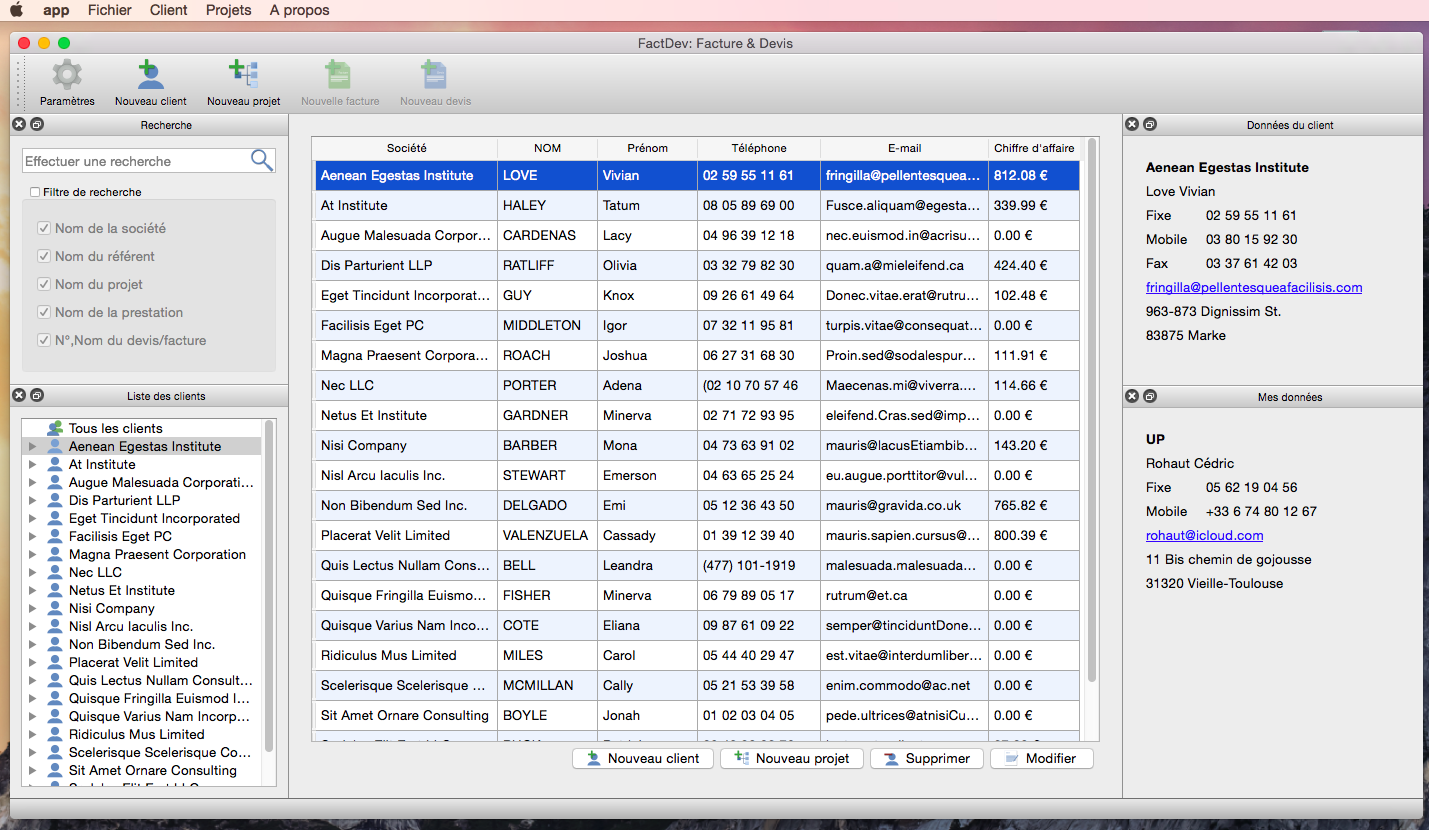
\includegraphics[height=5.5cm]{images/screens/mainWindow.png}~
		\caption{La fenêtre principale}
		}
		\only<2>{
		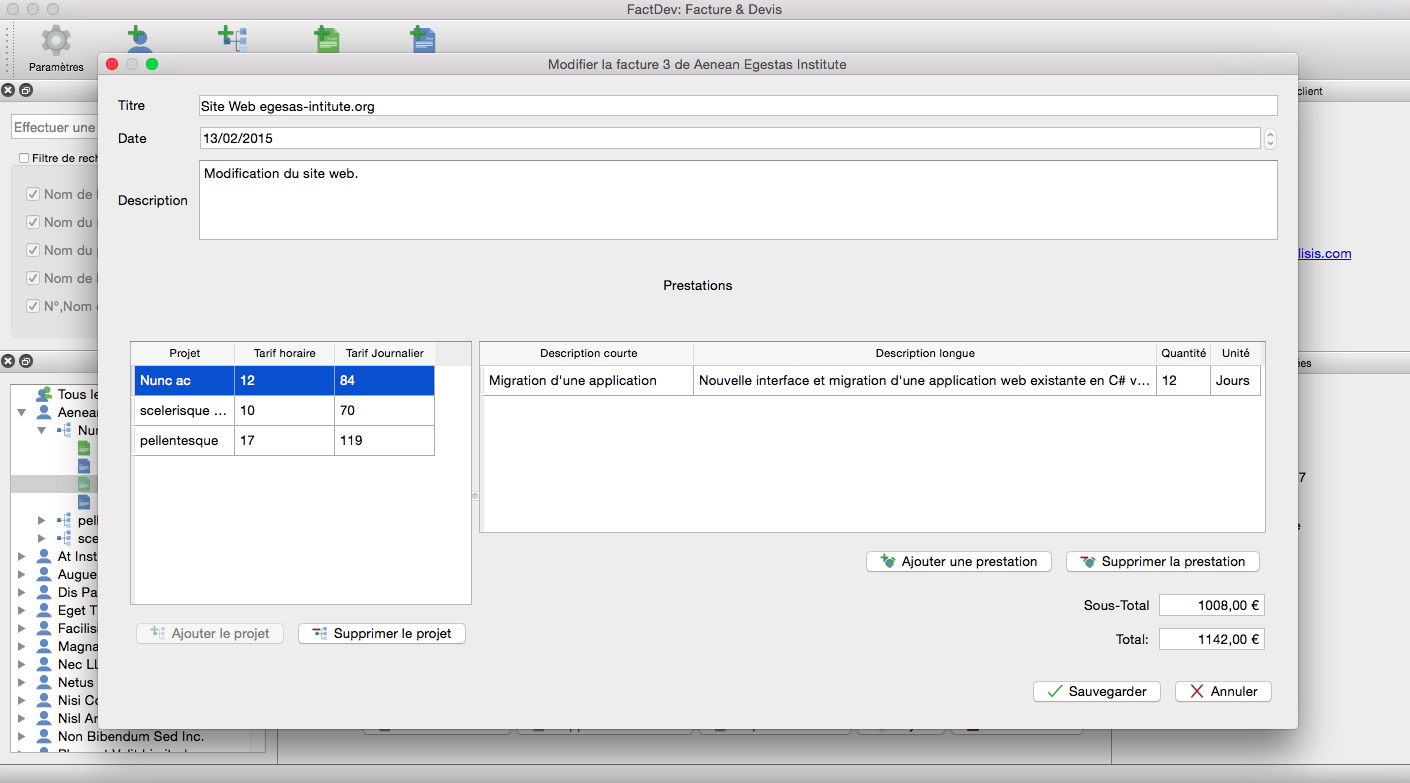
\includegraphics[height=5.5cm]{images/screens/editBill.png}~
		\caption{Édition d'une facture}
		}
		\only<3>{
		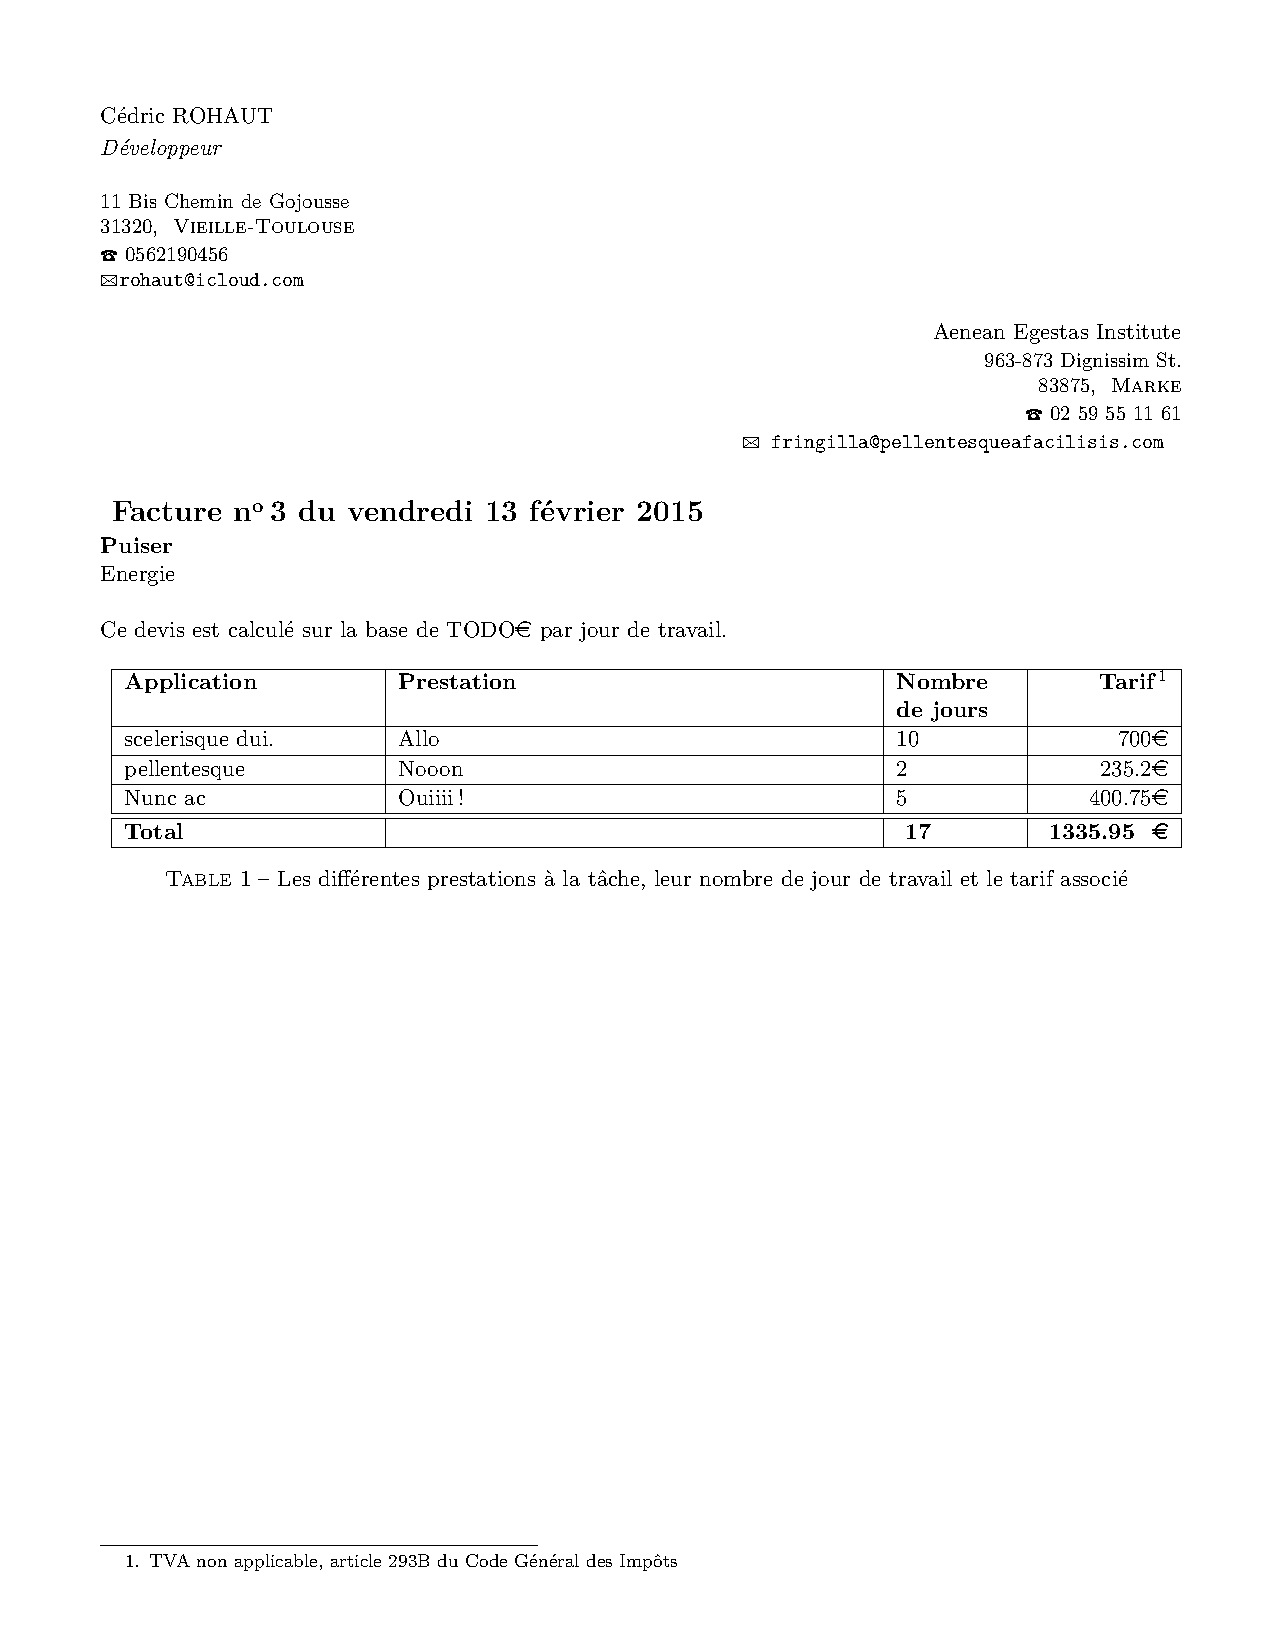
\includegraphics[height=5.5cm]{images/screens/facture.pdf}~
		\caption{Facture générée}
		}
		\only<1-3>{
		\vspace{-13px}
		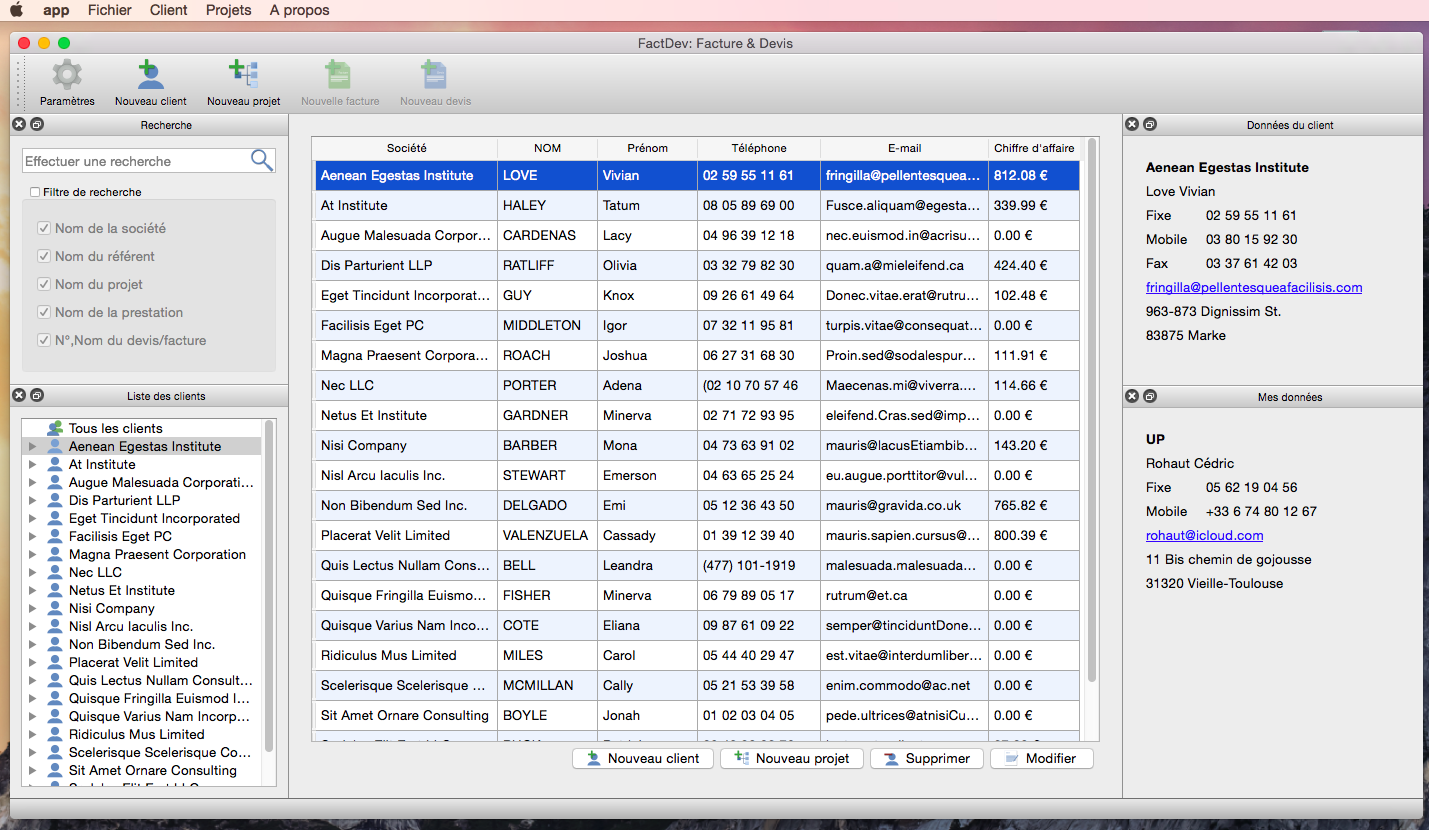
\includegraphics[height=1.5cm]{images/screens/mainWindow.png}~
		}
		\only<1>{
		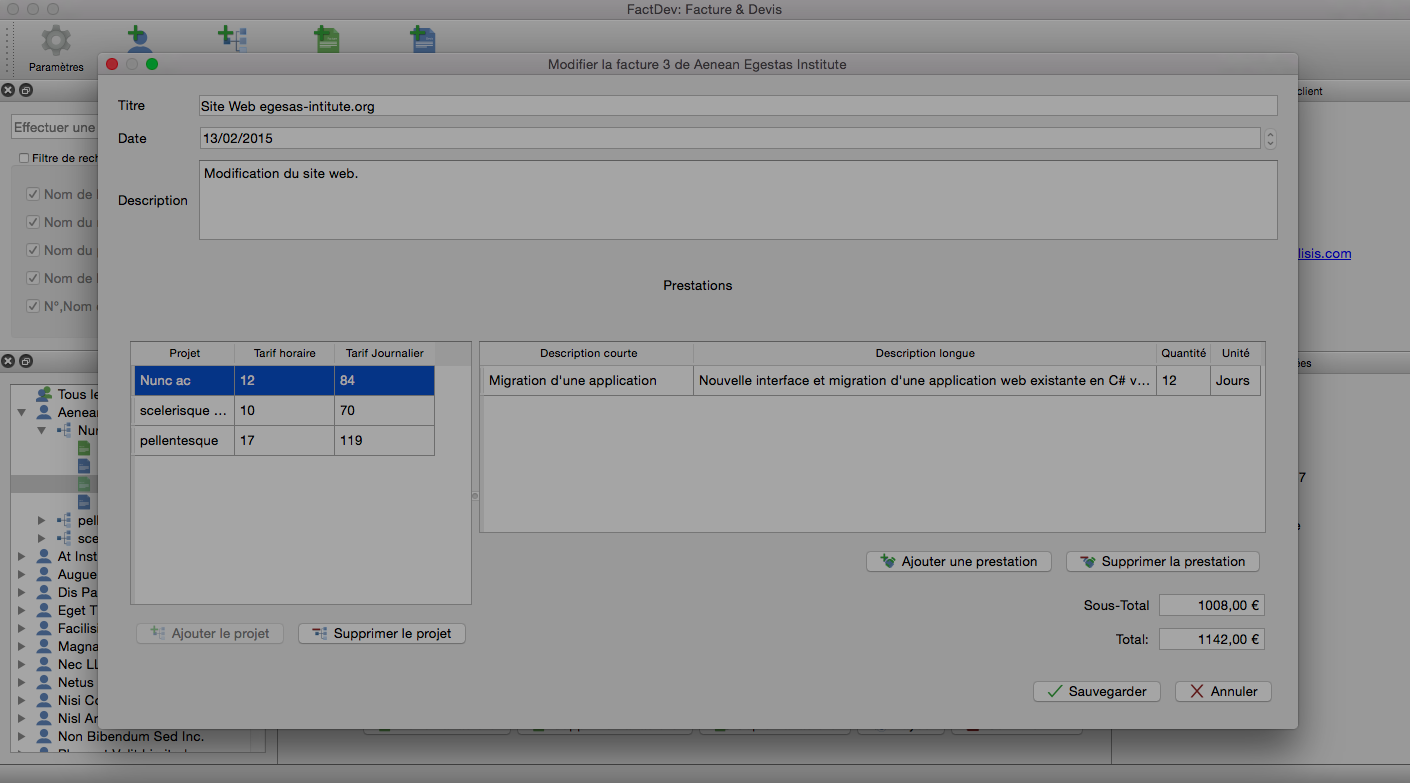
\includegraphics[height=1.5cm]{images/screens/editBill_grey.png}~
		}
		\only<2-3>{
		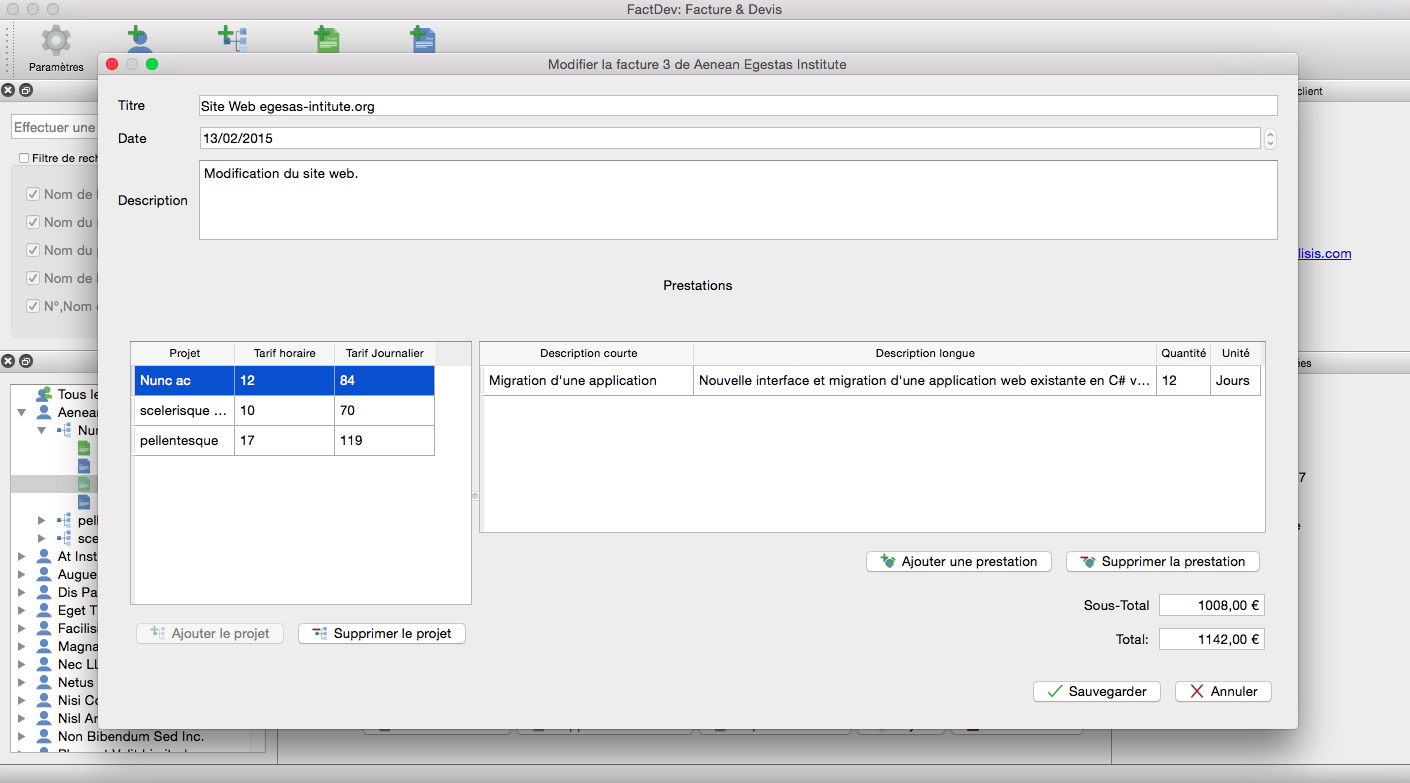
\includegraphics[height=1.5cm]{images/screens/editBill.png}~
		}
		\only<1-2>{
		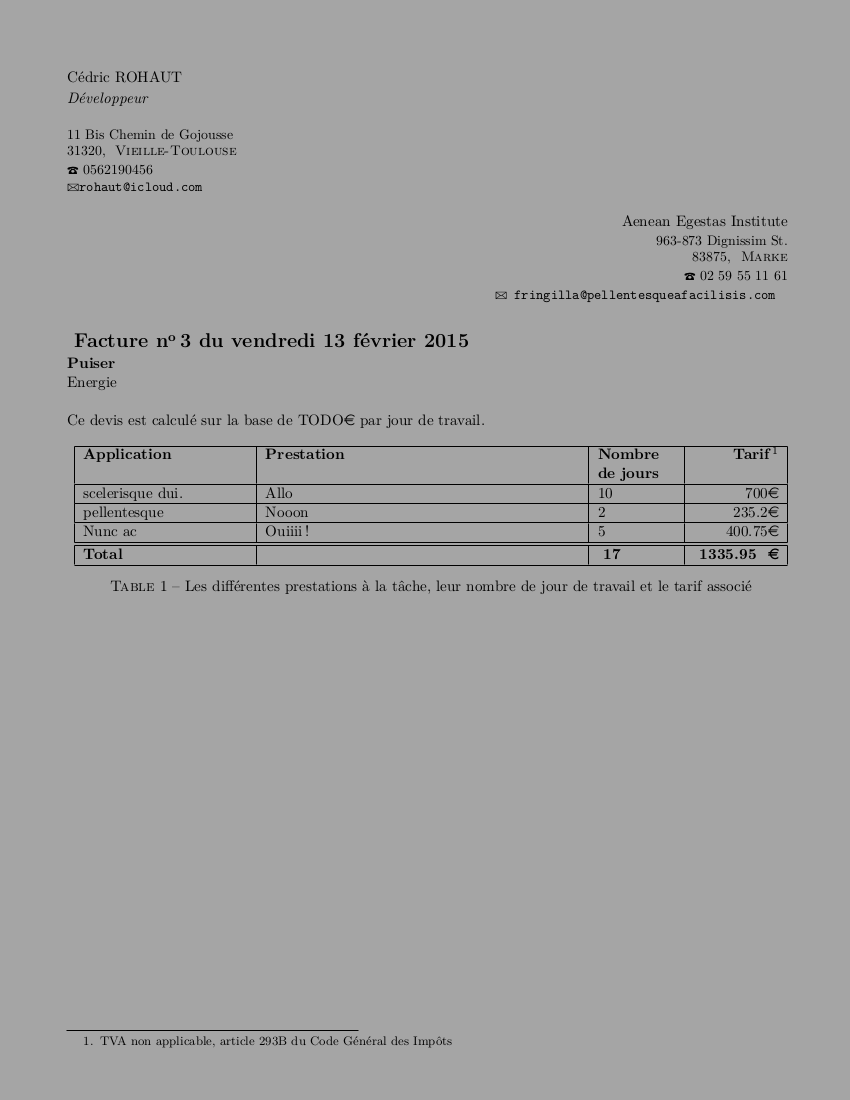
\includegraphics[height=1.5cm]{images/screens/facture_grey.png}
		}
		\only<3>{
		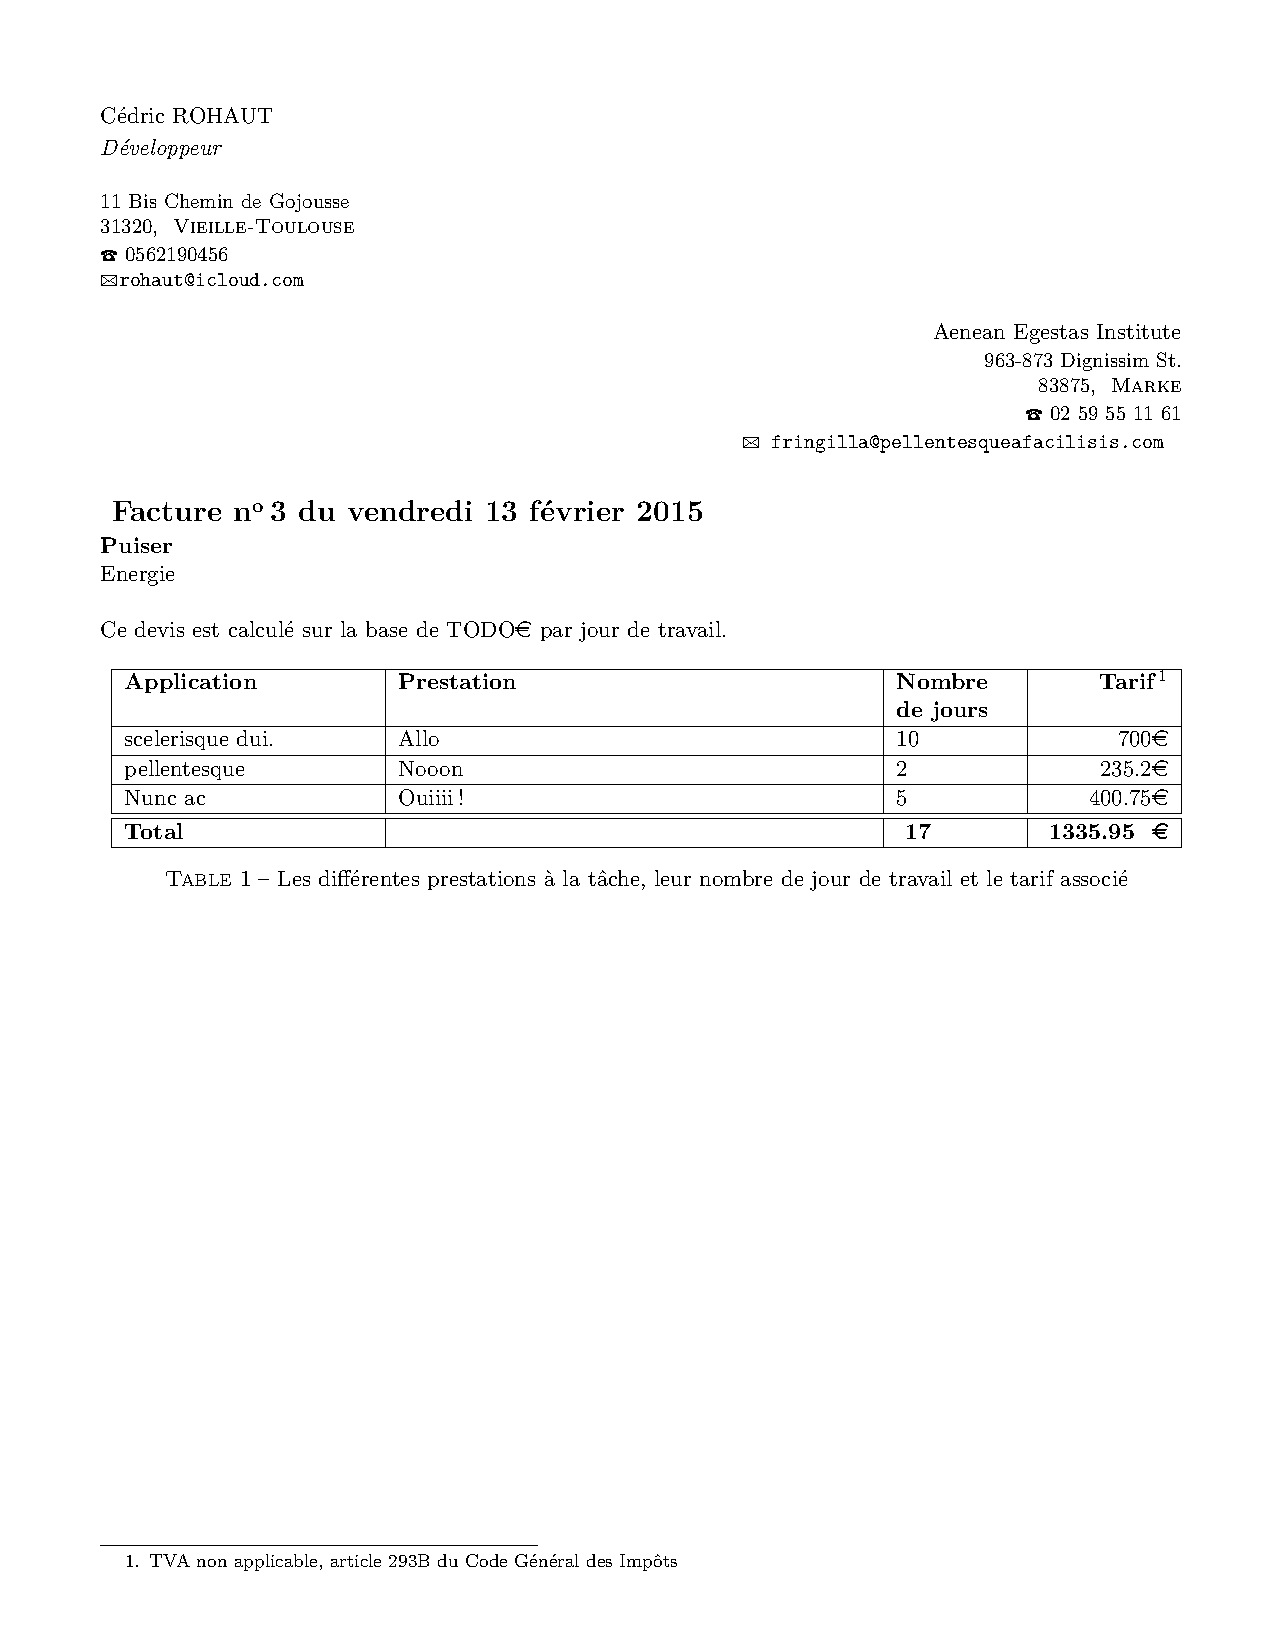
\includegraphics[height=1.5cm]{images/screens/facture.pdf}
		}
	\end{figure}
	\vfill

%	\only<1-7>{

%	\only<1-7>{
%	\begin{figure}[H]
%		\centering
%	}
%		\only<1>{
%		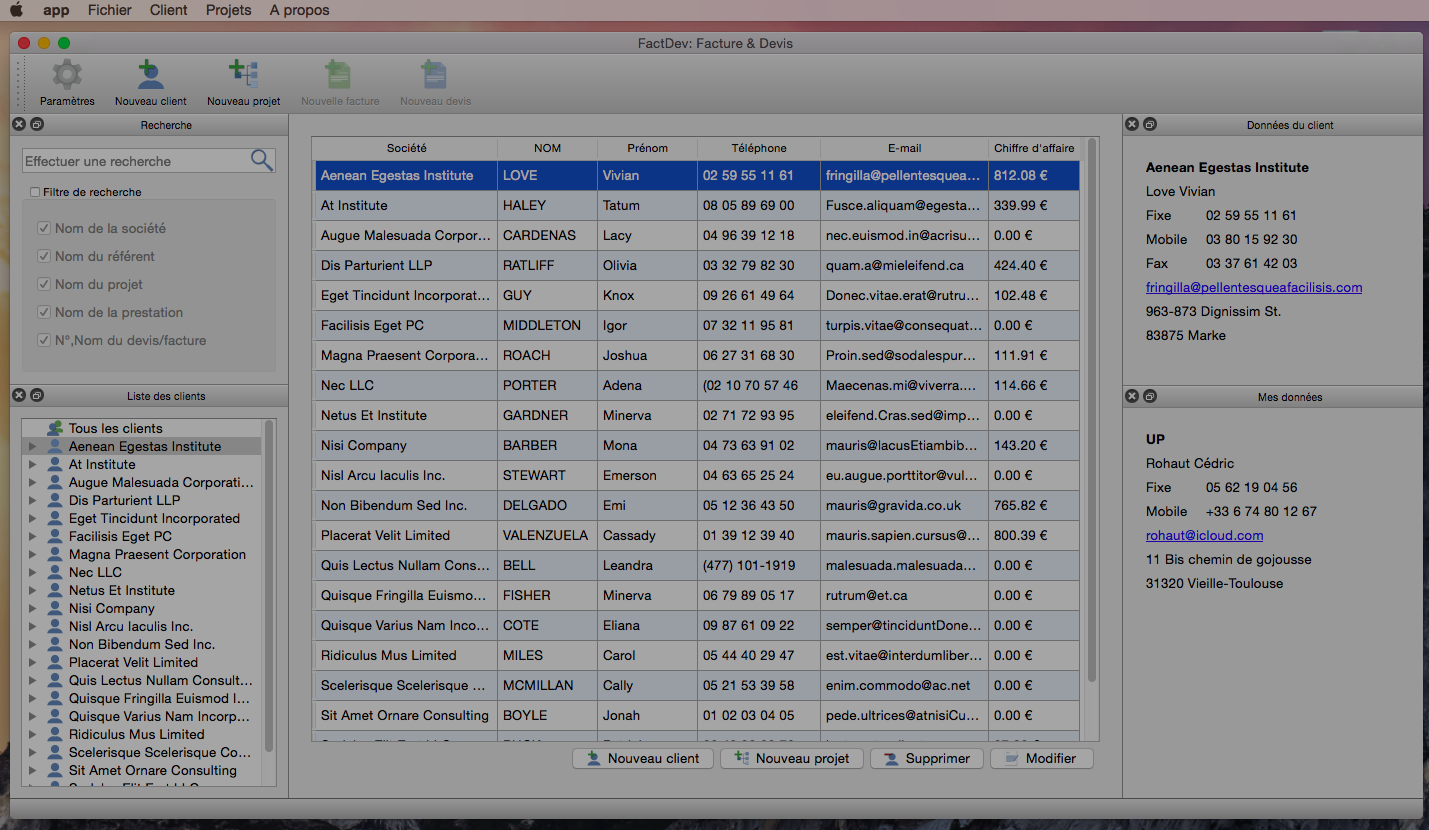
\includegraphics[width=4.5cm]{images/screens/mainWindow_grey.png}~
%		}
%		\only<2-7>{
%		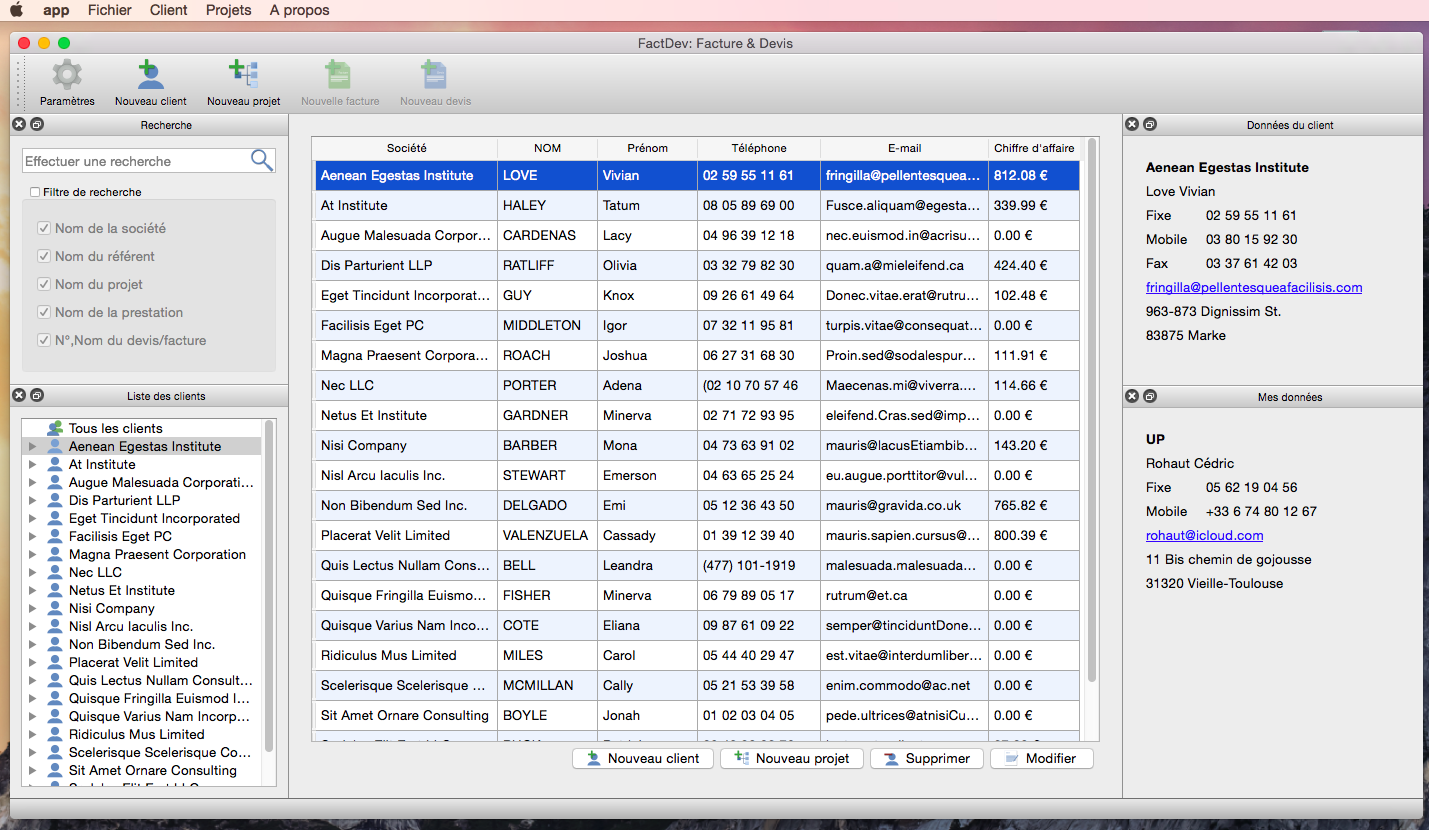
\includegraphics[width=4.5cm]{images/screens/mainWindow.png}~
%		}
%		\only<1-3>{
%		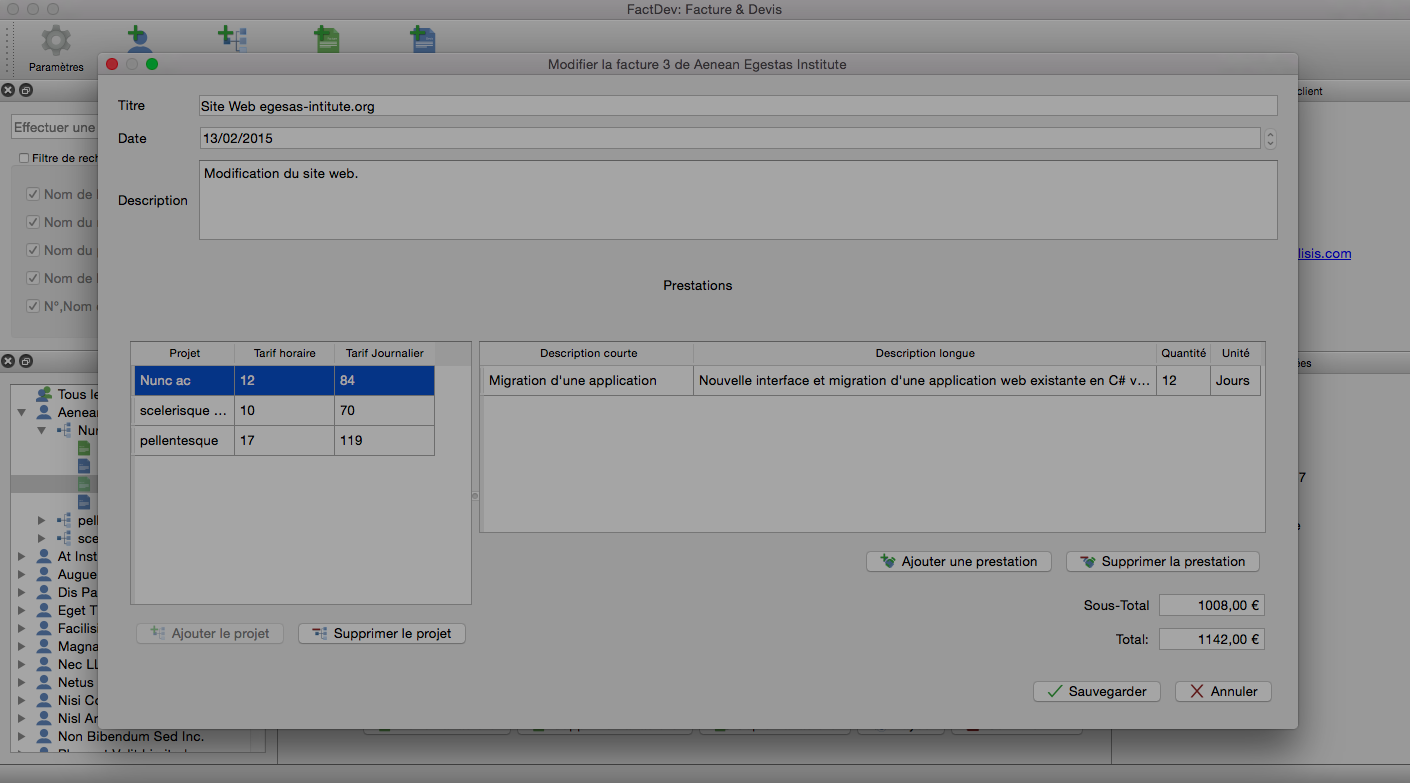
\includegraphics[width=4.5cm]{images/screens/editBill_grey.png}~
%		}
%		\only<4-7>{
%		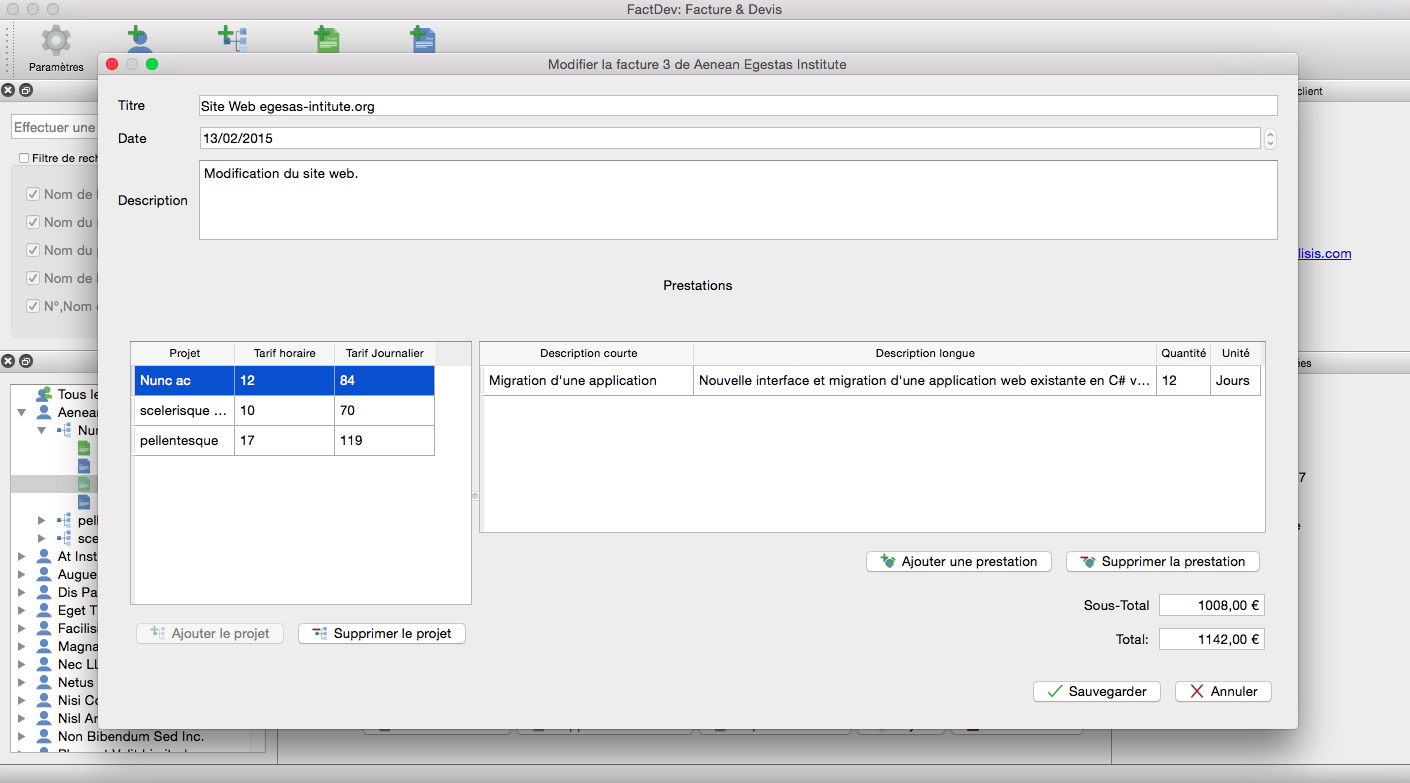
\includegraphics[width=4.5cm]{images/screens/editBill.png}~
%		}
%		\only<1,3,5>{
%		\newline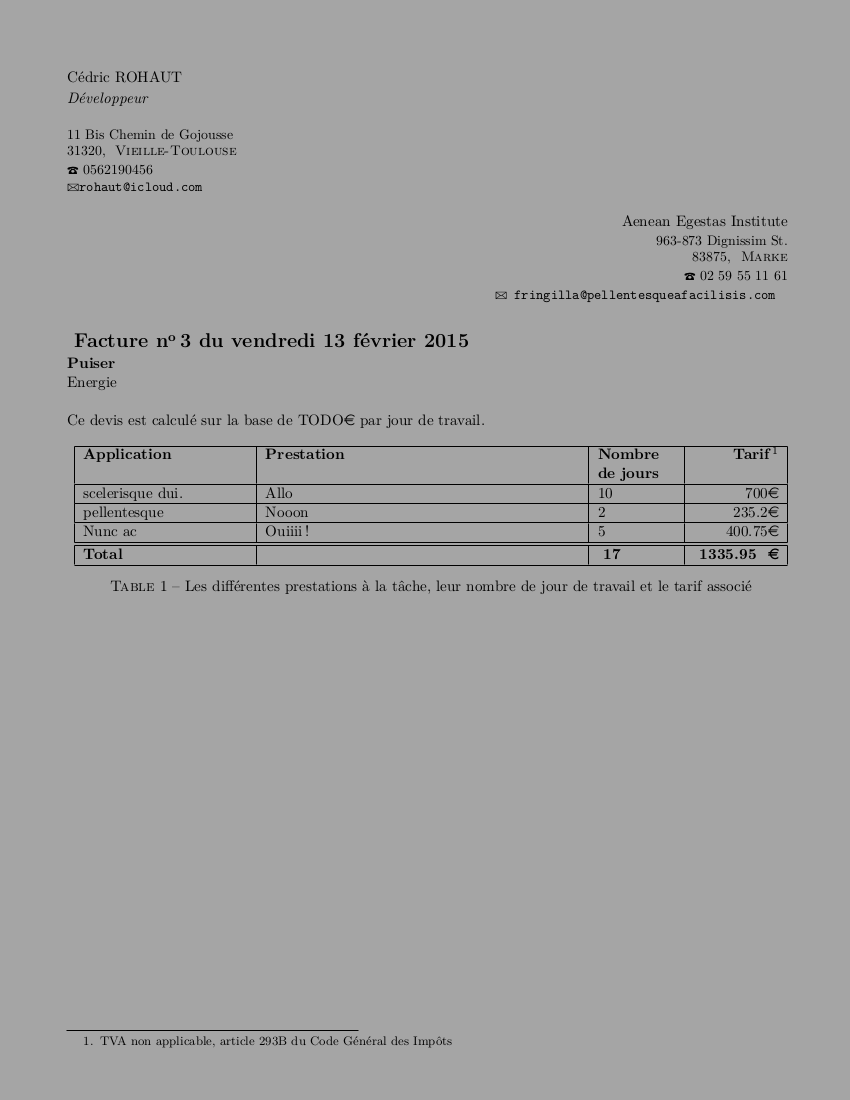
\includegraphics[width=3cm]{images/screens/facture_grey.png}
%		}
%		\only<7>{
%		\newline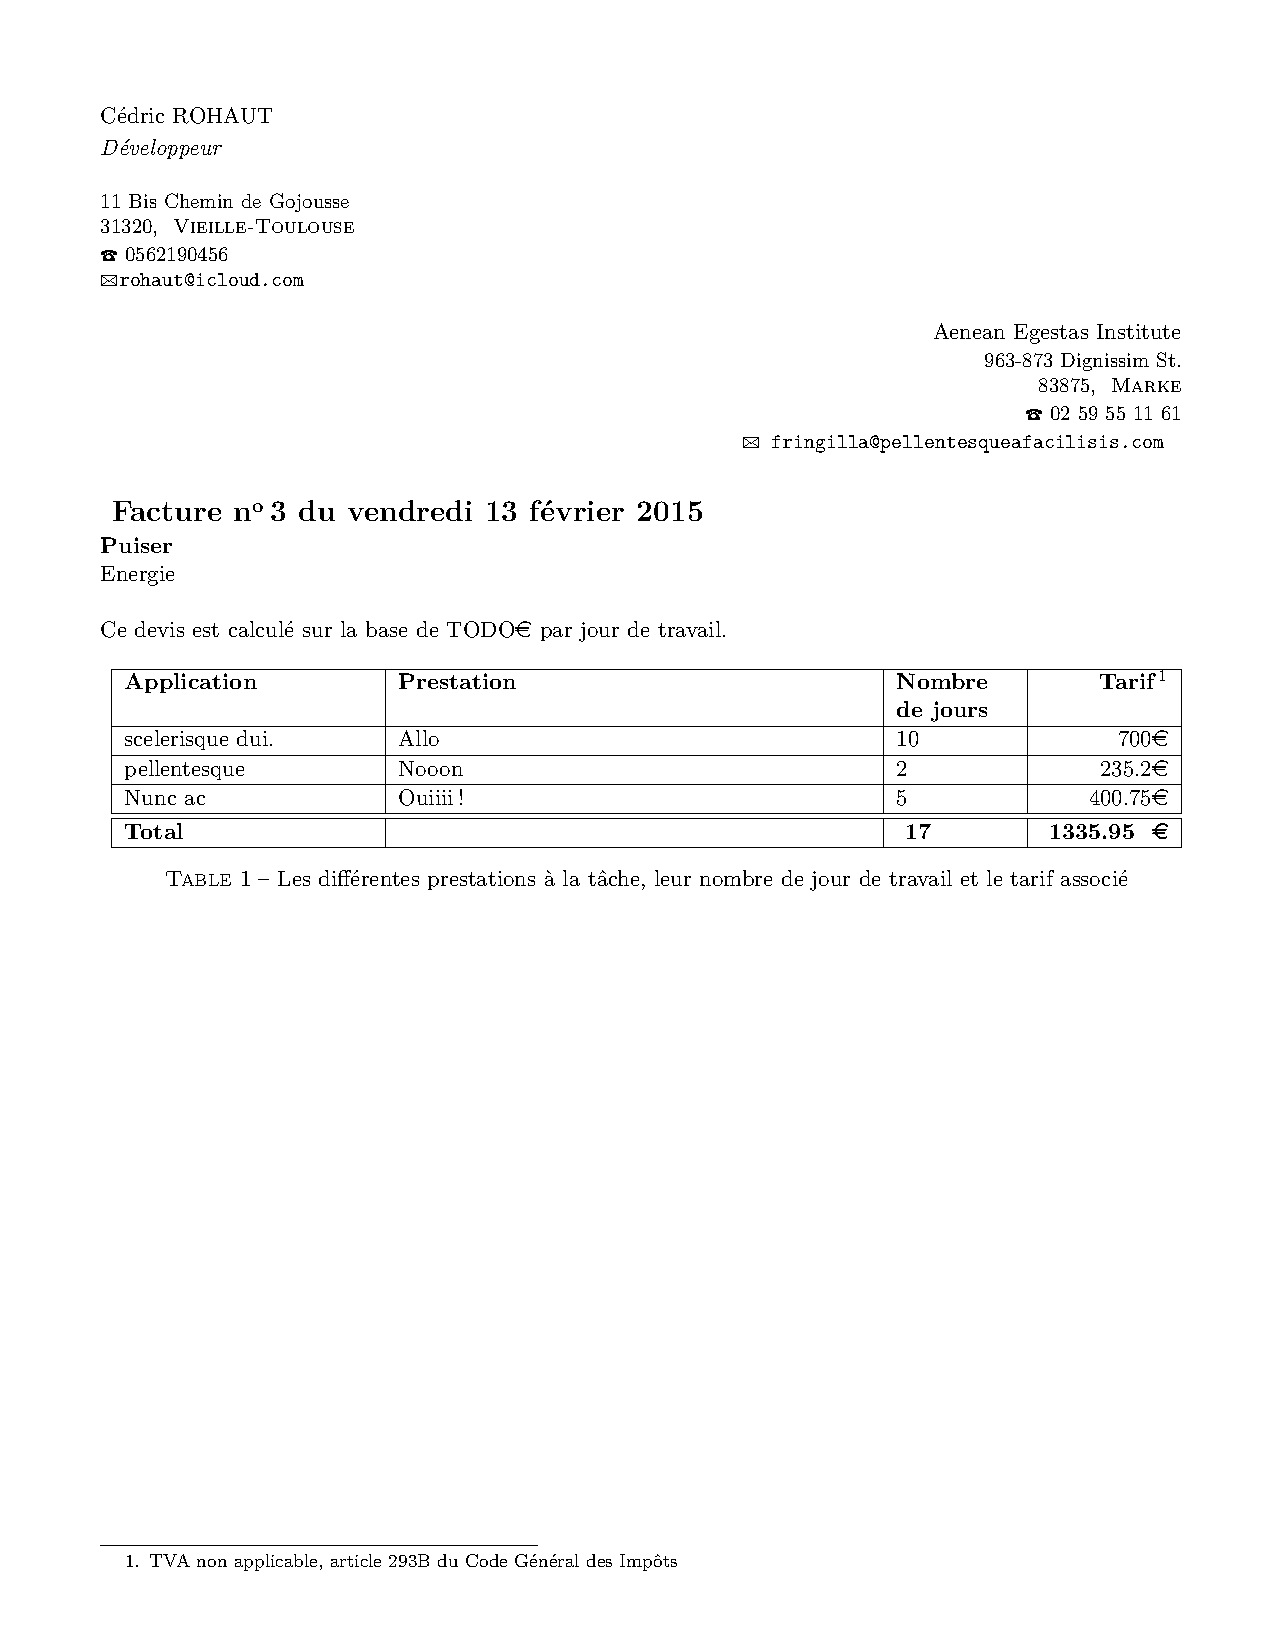
\includegraphics[width=3cm]{images/screens/facture.pdf}
%		}
%		\only<1,3,5,7>{
%		\caption{Les différentes captures d'écrans}
%		}
%	\only<1-7>{
%	\end{figure}
%	}

%	\only<4> {
%	\vspace{-3cm}
	%\begin{figure}[H]
	%	\centering
	%	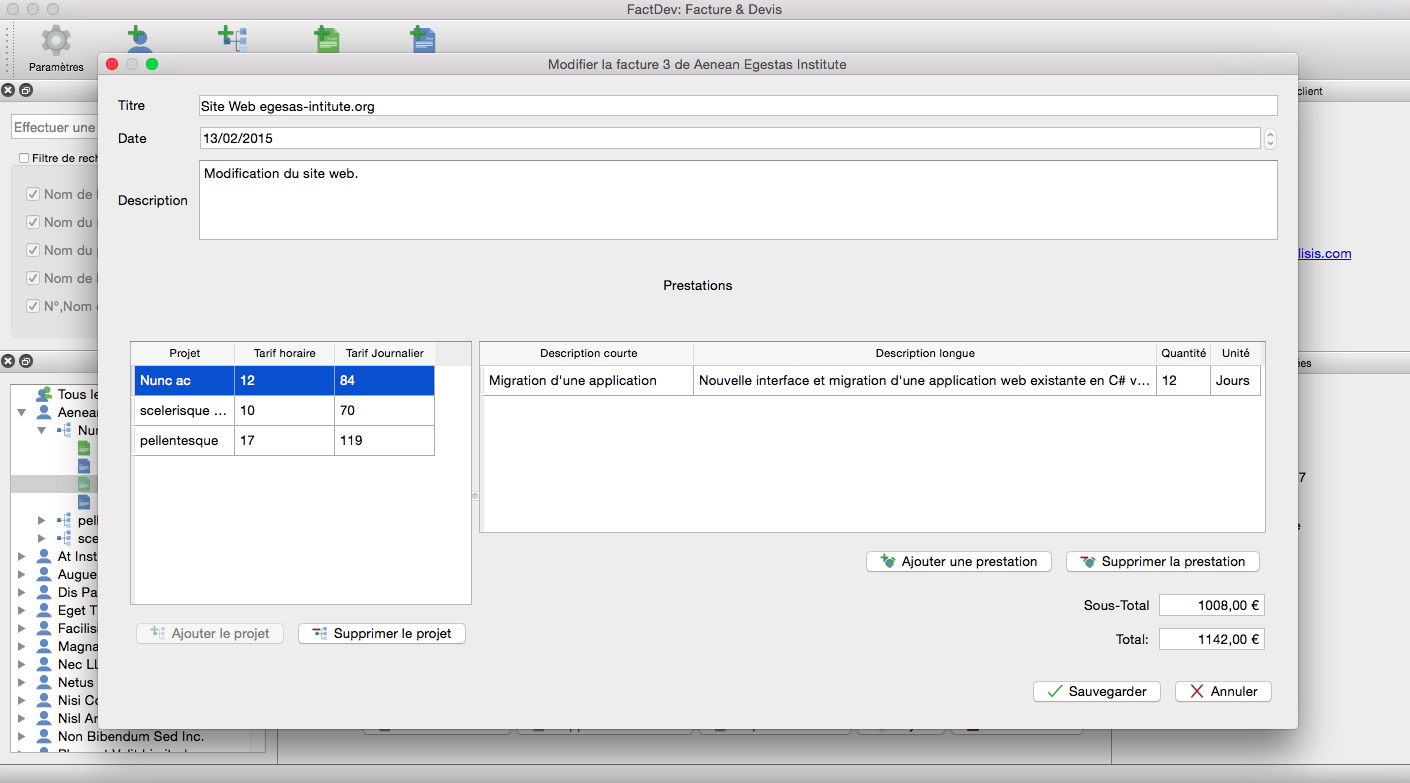
\includegraphics[width=9cm]{images/screens/editBill.png}~
	%	\caption{L'édition d'une facture}
%	\end{figure}
%	}
%	\only<6> {
%	\vspace{-3cm}
%	\begin{figure}[H]
%		\centering
%		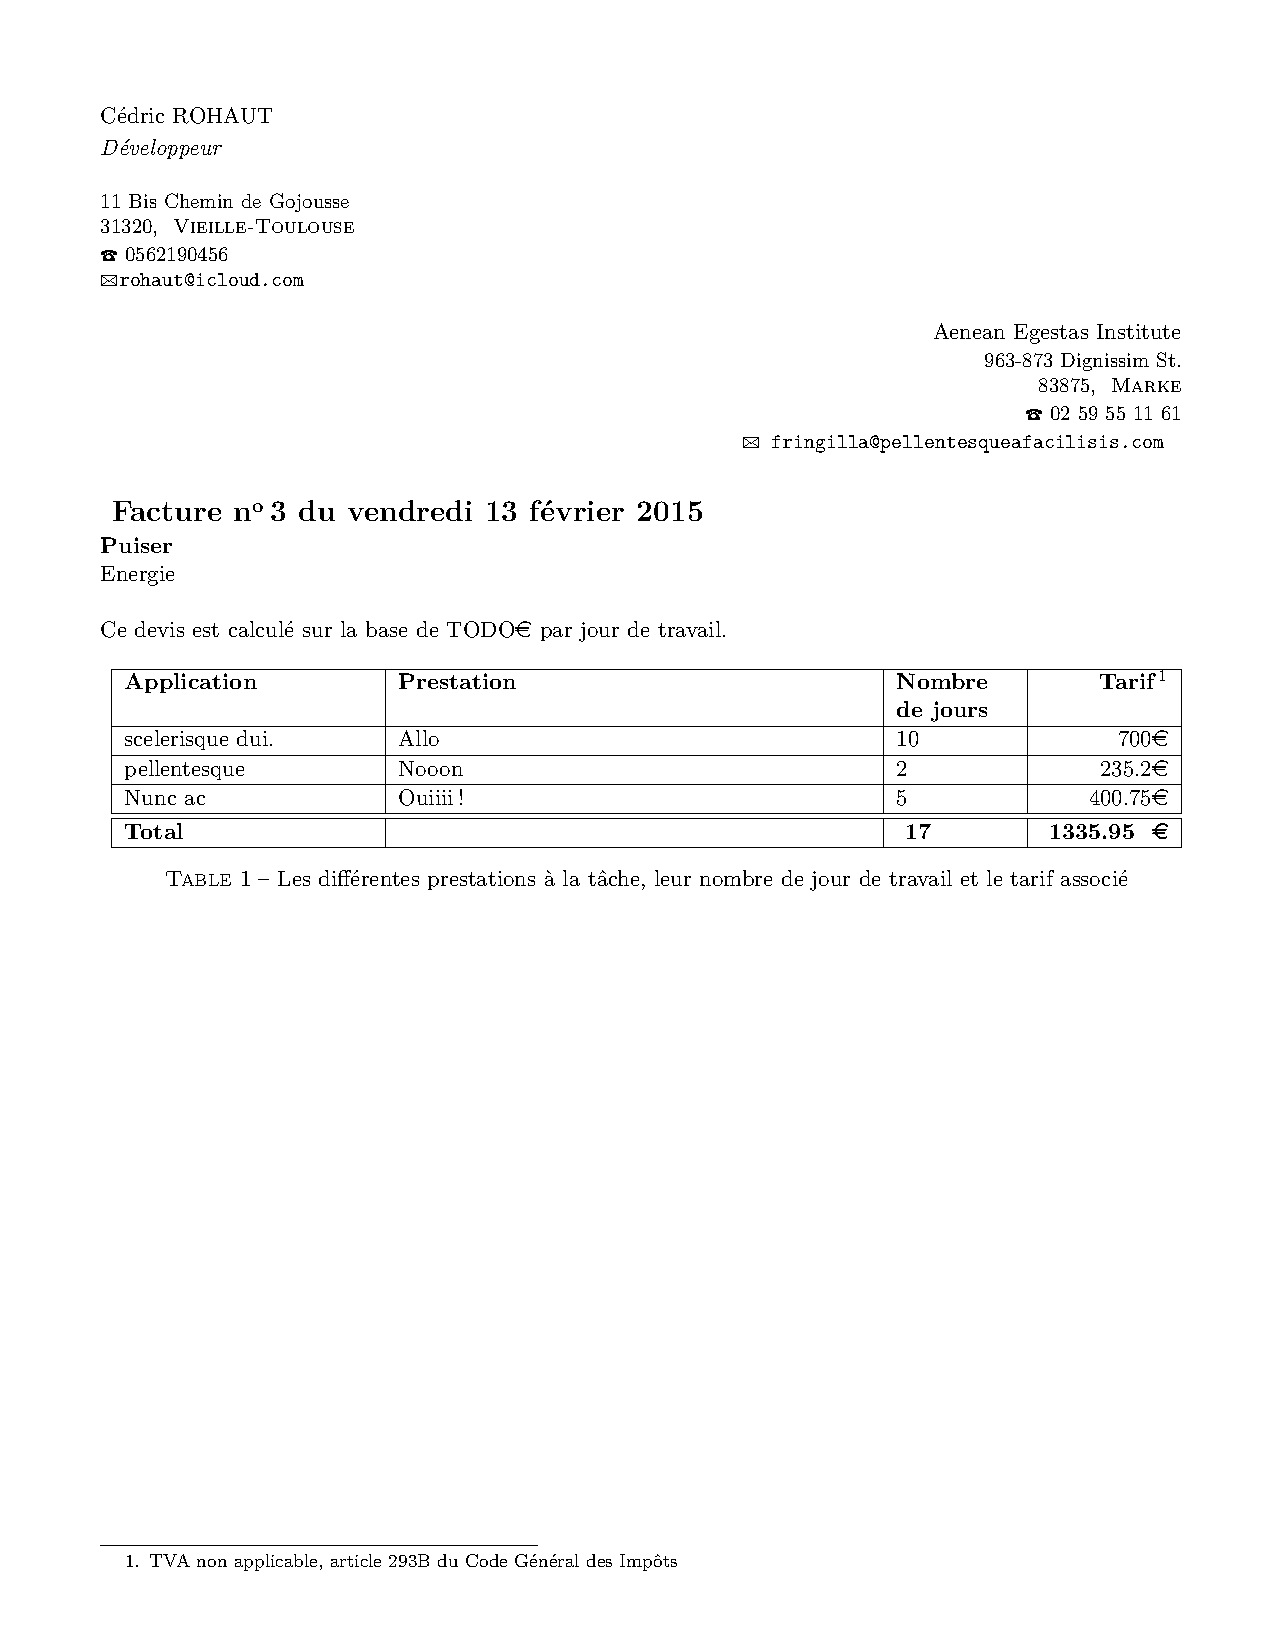
\includegraphics[width=5cm]{images/screens/facture.pdf}~
%		\caption{Un exemple de facture générée}
%	\end{figure}
%	}

\end{frame}

